%%%%%%%%%%%%%%%%%%%%%%%%%%%%%%%%%%%%%%%%%%%%%%%%%%%%%%%%%%%% 
% Name: XeTeX+xeCJK日常使用模板
% Author: Lox Freeman
% Email: xiaohanyu1988@gmail.com
% 、
% 本文档可以自由转载、修改,希望能给广大TeXer的中文之路提供一些方便。
%%%%%%%%%%%%%%%%%%%%%%%%%%%%%%%%%%%%%%%%%%%%%%%%%%%%%%%%%%%% 

\documentclass[a4paper, 12pt, titlepage]{article}

%%%%%%%%%%%%%%%%%%%%%%%%% xeCJK相关宏包%%%%%%%%%%%%%%%%%%%%%%%%%
\usepackage{xltxtra,fontspec,xunicode}
\usepackage[slantfont, boldfont, CJKchecksingle]{xeCJK}

\CJKsetecglue{\hskip 0.15em plus 0.05em minus 0.05em}
% slanfont: 允许斜体
% boldfont: 允许粗体
% CJKnormalspaces: 仅忽略汉字之间的空白,但保留中英文之间的空白。
% CJKchecksingle: 避免单个汉字单独占一行。
% CJKaddspaces: [备选]忽略汉字之间的空白,并且自动在中英文转换时插入空白。

% \CJKlanguage{zh-cn}                 % 中文标点特殊处理
\XeTeXlinebreaklocale "zh"           % 针对中文进行断行
\XeTeXlinebreakskip = 0pt plus 1pt minus 0.1pt
% 给予TeX断行一定自由度
%%%%%%%%%%%%%%%%%%%%%%%%% xeCJK%%%%%%%%%%%%%%%%%%%%%%%%%%%%%%%%

%%%%%%%%%%%%% 日常所用宏包、通通放在一起%%%%%%%%%%%%%%%%%%%%%%%%%%%%
% 什么常用的宏包都可以放这里。下面是我常用的宏包,每个都给出了简要注释
\usepackage[top=2.5cm, bottom=3cm, left=2.5cm, right=2.5cm]{geometry} % 控制页边距
\usepackage{enumerate}               % 控制项目列表
\usepackage{multicol}                % 多栏显示

\usepackage[%
pdfstartview=FitH,%
CJKbookmarks=true,%
bookmarks=true,%
bookmarksnumbered=true,%
bookmarksopen=true,%
colorlinks=true,%
citecolor=seco,%
linkcolor=seco,%
anchorcolor=seco,%
urlcolor=seco%
]{hyperref}                          % 超链接相关设置

\usepackage{titlesec}                % 控制标题
\usepackage{titletoc}                % 控制目录
\usepackage{type1cm}                 % 控制字体大小
\usepackage{indentfirst}             % 首行缩进,用\noindent取消某段缩进
\usepackage{bbding}                  % 一些特殊符号
\usepackage{cite}                    % 支持引用
\usepackage{framed,color,xcolor}     % 支持彩色文本、底色、文本框等
\usepackage{latexsym}                % LaTeX一些特殊符号宏包
\usepackage{amsmath}                 % AMS LaTeX宏包
\usepackage{bm}                      % 数学公式中的黑斜体
\usepackage{relsize}                 % 调整公式字体大小:\mathsmaller, \mathlarger
\usepackage{soul}                    % 下划线自动回车换行
\usepackage{attachfile}              % 添加附见使用的宏包
\usepackage{parcolumns}              % 列排版
\usepackage{framed}
\usepackage{tcolorbox}
\usepackage{pdfpages}                % 直接引用已有的PDF文件
\usepackage{soul}                    % 自动换行的下划线
\makeindex                           % 生成索引

\makeatletter
\let\std@footnotetext\@footnotetext
\usepackage{setspace}
\let\@footnotetext\std@footnotetext
\makeatother

%%%%%%%%%%%%%%%%%%%%%%%%% 绘图方法%%%%%%%%%%%%%%%%%%%%%%%%%%%
\usepackage{graphicx}                % 图形宏包
\graphicspath{{./figure/}{./figures/}{./image/}{./graphics/}{./graphic/}{./pictures/}{./picture/}}

\usepackage{tikz}
\usepackage{amsmath,bm,times}
\usepackage{verbatim}

\usepackage{tabularx}

\usetikzlibrary{shapes,arrows,shadows,fit,snakes,positioning,decorations}
\usetikzlibrary{decorations.shapes}
\usetikzlibrary{calc}           %coordinate

\usepackage{caption}
\usepackage{float}

\ifx\du\undefined
\newlength{\du}
\fi
\setlength{\du}{15\unitlength}

\newlength\Textwd
\setlength\Textwd{3cm}
\newcommand\Textbox[2]{%
  \parbox[c][#1][c]{\Textwd}{\linespread{0.5}\centering#2}}

\makeatletter
\DeclareRobustCommand{\rvdots}{%
  \vbox{
    \baselineskip6\p@\lineskiplimit\z@
    \kern-\p@
    \hbox{.}\hbox{.}\hbox{.}
  }}
\makeatother


\makeatletter
\DeclareRobustCommand{\rvdots}{%
  \vbox{
    \baselineskip4\p@\lineskiplimit\z@
    \kern-\p@
    \hbox{.}\hbox{.}\hbox{.}}}
\tikzset{
  heights/.code={
    \def\pgf@tempb{}%
    \foreach \qrr@tikz@rs@height[count=\qrr@tikz@count from 1] in {#1}{
      \edef\pgf@tempa{\noexpand\pgfkeysalso{/tikz/every \pgf@lib@sh@toalpha\qrr@tikz@count\space node part/.append style={height={\qrr@tikz@rs@height}}}}%
      \ifnum\qrr@tikz@count=1\relax % allows to use \nodepart{text} (or not at all for the first part)
      \edef\pgf@tempa{\unexpanded\expandafter{\pgf@tempa}\noexpand\pgfkeysalso{/tikz/every text node part/.append style={height={\qrr@tikz@rs@height}}}}%
      \fi
      \expandafter\pgfutil@g@addto@macro\expandafter\pgf@tempb\expandafter{\pgf@tempa}
    }
    \pgf@tempb
  },
  height/.code={%
    \expandafter\def\expandafter\pgfutil@minipage\expandafter[\expandafter##\expandafter 1\expandafter]\expandafter{\pgfutil@minipage[][#1][c]}% LaTeX only!
  }
}

\makeatother
\tikzset{rect/.style={
    draw,
    rectangle split,
    rectangle split parts=1,
    rectangle split part align=center,
    draw,
    % font=\ttfamily, % still works
    thick,
    text width=2.5cm,
    align=center,
    rectangle split part align={center,left,right},
    % rectangle split part fill={PaleTurquoise1},
  }}

\makeatletter
\newcommand{\gettikzxy}[3]{%
  \tikz@scan@one@point\pgfutil@firstofone#1\relax
  \edef#2{\the\pgf@x}%
  \edef#3{\the\pgf@y}%
}
\makeatother
%%%%%%%%%%%%%%%%%%%%%%%%% 绘图方法结束%%%%%%%%%%%%%%%%%%%%%%%%%%%

%%%%%%%%%%%%%%%%%%%%%%%%% fancyhdr设置页眉页脚%%%%%%%%%%%%%%%%%%%%
\usepackage{etoolbox}
\usepackage{fancyhdr}                % 页眉页脚
\pagestyle{fancy}                    % 页眉页脚风格
\setlength{\headheight}{15pt}        % 有时会出现\headheight too small的warning

\makeatletter
\patchcmd{\@fancyhead}{\rlap}{\color{seco}\rlap}{}{}
\patchcmd{\headrule}{\hrule}{\color{seco}\hrule}{}{}
\patchcmd{\@fancyfoot}{\rlap}{\color{seco}\rlap}{}{}
\patchcmd{\footrule}{\hrule}{\color{seco}\hrule}{}{}
\makeatother
%%%%%%%%%%%%%%%%%%%%%%%%% fancyhdr设置结束%%%%%%%%%%%%%%%%%%%%%%%

%%%%%%%%%%%%%%%%%%%%%%%%% xeCJK字体设置%%%%%%%%%%%%%%%%%%%%%%%%%
% \setmainfont[Ligatures=TeX]{Minion Pro} % (\textrm)
\setmainfont[Ligatures=TeX]{Calibri} % (\textrm)
% \setsansfont{Myriad Pro}                % (\textsf)
\setsansfont{Calibri}                % (\textsf)
% \setmonofont{Adobe Garamond Pro}        % Palatino Linotype
\setmonofont{Ubuntu Mono}        % Palatino Linotype

\setCJKmainfont[BoldFont={方正兰亭纤黑_GBK},ItalicFont={Adobe Kaiti Std}]{Adobe Kaiti Std}
\setCJKsansfont[BoldFont={方正兰亭纤黑_GBK}]{方正兰亭纤黑_GBK}
\setCJKmonofont{方正兰亭纤黑_GBK}
%%%%%%%%%%%%%%%%%%%%%%%%% xeCJK字体设置结束%%%%%%%%%%%%%%%%%%%%%%

%%%%%%%%%%%%%%%%%%%%%%%%% listings宏包粘贴源码%%%%%%%%%%%%%%%%%%%%
\usepackage{listings}                % 方便粘贴源代码,部分代码高亮功能
\lstloadlanguages{}                  % 所要粘贴代码的编程语言

\newfontfamily\listingsfont{Ubuntu Mono}
\newfontfamily\listingsfontinline{Calibri}

\definecolor{sh_keyword}{rgb}{0.06, 0.10, 0.98}   % #101AF9
\definecolor{shadecolor}{rgb}{0.83, 0.83, 0.83}
\definecolor{monokai-grey-dark}{RGB}{39, 40, 34}   % #272822
\definecolor{monokai-yellow-light}{RGB}{248, 248, 246}   % #F8F8F2
\definecolor{monokai-green}{RGB}{166, 226, 42}
\definecolor{dark green}{rgb}{0.000000,0.392157,0.000000}
\definecolor{forest green}{rgb}{0.133333,0.545098,0.133333}
\def\lstsmallmath{\leavevmode\ifmmode \scriptstyle \else  \fi}
\def\lstsmallmathend{\leavevmode\ifmmode  \else  \fi}

% \definecolor{seco}{RGB}{9,80,3}
% \definecolor{seco}{RGB}{0,145,215}
\definecolor{seco}{RGB}{0,175,152}
\definecolor{main}{RGB}{127,191,51}

% \makeatletter
%   \newcommand\listingfont{\@setfontsize\listingfont{11pt}{13.2pt}}
% \makeatother

\renewcommand{\lstlistingname}{代码}

\lstset {
  language=c++,
  backgroundcolor=\color{monokai-grey-dark},
  % frame=shadowbox,
  % breaklines,
  % rulesepcolor=\color{red!20!green!20!blue!20},
  showspaces=false,showtabs=false,tabsize=4,
  numberstyle=\tiny\color{black},numbers=left,
  % basicstyle= \listingfont\listingsfont\color{monokai-yellow-light},
  basicstyle= \small\listingsfont\color{monokai-yellow-light},
  stringstyle=\color{dark green},
  % keywordstyle = \color{monokai-green}\bfseries,
  keywordstyle = \color{monokai-green},
  commentstyle=\footnotesize\color{forest green}\itshape,
  captionpos=b,
  showspaces=false,showtabs=false, showstringspaces=false,
  xleftmargin=0.7cm, xrightmargin=0.5cm,
  % lineskip=-0.3em,
  breaklines=tr,
  escapebegin={\lstsmallmath}, escapeend={\lstsmallmathend},
  extendedchars=false
}

\lstnewenvironment{acol}[1][]{\lstset{language={[x86masm]Assembler},#1}}{}
\newenvironment{parcolumenv}[1] {\begin{spacing}{#1}}{\end{spacing}}
%%%%%%%%%%%%%%%%%%%%%%%%% listings宏包设置结束%%%%%%%%%%%%%%%%%%%%


%%%%%%%%%%%%%%%%%%%%%%%%% 一些关于中文文档的重定义%%%%%%%%%%%%%%%%%

%%%% 数学公式定理的重定义%%%%
\newtheorem{example}{例}                                   % 整体编号
\newtheorem{algorithm}{算法}
\newtheorem{theorem}{定理}[section]                        % 按 section 编号
\newtheorem{definition}{定义}
\newtheorem{axiom}{公理}
\newtheorem{property}{性质}
\newtheorem{proposition}{命题}
\newtheorem{lemma}{引理}
\newtheorem{corollary}{推论}
\newtheorem{remark}{注解}
\newtheorem{condition}{条件}
\newtheorem{conclusion}{结论}
\newtheorem{assumption}{假设}

%%%% 章节等名称重定义%%%%
\renewcommand{\contentsname}{目\hspace{2em}录}
\renewcommand{\indexname}{索引}
\renewcommand{\listfigurename}{插图目录}
\renewcommand{\listtablename}{表格目录}
\renewcommand{\figurename}{图}
\renewcommand{\tablename}{表}
\renewcommand{\appendixname}{附\hspace{2em}录}

%%%% 设置chapter、section与subsection的格式%%%%
\titleformat{\chapter}{\centering\huge}{\color{seco}第\thechapter{}章}{1em}{\color{seco}\textbf}
\titleformat{\section}{\centering\LARGE}{\color{seco}\thesection}{1em}{\color{seco}\textbf}
\titleformat{\subsection}{\Large}{\color{seco}\thesubsection}{1em}{\color{seco}\textbf}
%%%%%%%%%%%%%%%%%%%%%%%%% 中文重定义结束%%%%%%%%%%%%%%%%%%%%


%%%%%%%%%%%%%%%%%%%%%%%%% 一些个性设置%%%%%%%%%%%%%%%%%%%%%%
\setlength{\parskip}{0.5\baselineskip}     % 设定段间距
\linespread{1.6}                           % 设定行距
\newcommand{\pozhehao}{\kern0.3ex\rule[0.8ex]{2em}{0.1ex}\kern0.3ex}% 中文破折号,据说来自清华模板

\setCJKfamilyfont{title}{方正正中黑简体}

\newcommand*{\TitleFont}{\usefont{\encodingdefault}{\rmdefault}{b}{n}\fontsize{32}{40}\selectfont\CJKfamily{title}\color{seco}}% 标题字体设置

\renewcommand{\today}{\color{seco}\number\year 年 \number\month 月 \number\day 日}
%%%%%%%%%%%%%%%%%%%%%%%%% 个性设置结束%%%%%%%%%%%%%%%%%%%%%%


%%%%%%%%%%%%%%%%%%%%%%%%% 正文部分%%%%%%%%%%%%%%%%%%%%%%%%%
\begin{document}
\setlength{\parindent}{2em}
% 设定首行缩进为2em。注意此设置一定要在document环境之中。
% 这可能与\setlength作用范围相关

\title{\TitleFont 由安全函数整改想到的\vspace{8cm}}
\author{\href{mailto:q00148943@gmail.com}{\LARGE{秦新良}}}
\date{\vspace{0.5cm}\today}

\maketitle

\tableofcontents
\newpage


\section{问题提出}
前段时间做安全函数整改,有部分文件未整改彻底,最近由赵阳同学接手将剩余遗留的非安全函数清理干净。在评审整改后的代码时,我对代码\ref{lst1}的修改\footnote{代码\ref{lst1}中的注释处即修改点。}方案提出了如下检视意见:
\begin{itemize}
\item pgwlib.h是BE发布给FE的头文件,不应该在该头文件中包含uscdbcommon.h;
\item USCDB\_MEMSET宏对FE不可见,不能在这里使用该宏定义,否则FE切换版本后会导致lib库编译失败。
\end{itemize}
针对以上两点检视意见,我给出的解决方法是:将类DataNode的构造函数挪到pgwlib.cpp文件中,这样即解决了安全问题,也不会对FE的lib库有任何影响。
\begin{spacing}{1.0}
  \lstinputlisting[label=lst1,caption=pgwlib.h]{list/pgwlib.h}
\end{spacing}
这一切看似很完美,但过了一会儿,赵阳发eSpace说,这样改不行,如果lib库中有该类的实例,实例化时会失败,因为找不到类DataNode构造函数的定义。

看了这样的回复觉得很“无语\footnote{无语归无语,但不得不说赵阳同学的基本功还是很扎实,能一眼看出问题之所在。}”。这不就是找一个函数地址吗,lib库被PGW加载后,和PGW是在同一进程地址空间内的,为什么会找不到PGW定义的函数?

支撑我这一想法的,除了lib库最终加载后和PGW在同一进程地址空间外,还有就是在该类整改前,DataNode的构造函数会调用memset函数和string的构造函数,这两个函数分别来自libc和libstdc++库。在编译lib库时,lib库看到的也只是标准库的头文件,并不会真正的把这两个标准库链接到动态库中,最终lib库中在有使用到memset或string的相关函数时,使用的也还是PGW进程加载起来的且和PGW在同一地址空间的标准库中的函数。那么lib库能找得到PGW加载起来的标准库中定义的函数,就能找的到PGW自己定义的函数。

但在冷静的分析之后,发现赵阳的说法也有一定道理。因为目前pgwlib.h头文件中定义的类,这些类的所有函数均是申明时就直接实现了,并没有放到任何一个cpp文件里。看了这样的实现后,决定写段代码来验证一下我的想法。

\section{问题验证}
验证的代码很简单,共三个源文件,见代码\ref{lst2}、代码\ref{lst3}和代码\ref{lst4}。

common.h模拟pgwlib.h。在common.h中定义类DataNode。该类有数据成员strData和除构造、析构函数外的成员函数printData。
\begin{spacing}{1.0}
  \lstinputlisting[label=lst2,caption=common.h]{list/common.h}
\end{spacing}

main.cpp模拟PGW。在该文件中除了实现main函数外,还完成了类DataNode相关函数的实现。
\begin{spacing}{1.0}
  \lstinputlisting[label=lst3,caption=main.cpp]{list/main.cpp}
\end{spacing}

datanode.cpp模拟FE的lib库,该文件包含了common.h头文件,并且定义了函数getNode,返回类DataNode的对象。
\begin{spacing}{1.0}
  \lstinputlisting[label=lst4,caption=datanode.cpp]{list/datanode.cpp}
\end{spacing}
模拟验证所需的源文件都已具备,执行如下两条命令即可生成可执行文件main和libdatanode.so动态库:
\begin{tcolorbox}[colback=green!5!white,colframe=orange]
  g++ -m32 -g -Wall main.cpp -o main -ldl\\
  g++ -m32 -g -Wall -shared -fPIC datanode.cpp -o libdatanode.so
\end{tcolorbox}
生成可执行文件和库文件后,按照之前的设想,运行main程序会打印出字符串"Hello world!",但实际执行的结果如下:
\begin{tcolorbox}[colback=green!5!white,colframe=orange]
  q00148943@Inspiron-3421:\char`\~\$ ./main
  \tcblower
  ./main: symbol lookup error: ./libdatanode.so: undefined symbol: \_ZN8DataNodeC1Ev
\end{tcolorbox}
符号\_ZN8DataNodeC1Ev用c++filt demangle后就是DataNode::DataNode(),即类DataNode的构造函数。也就是说,将pgwlib.h中类的构造及成员函数放到pgwlib.cpp文件中实现是行不通的。

虽然验证的结果是不可行的,但仍觉得这个结果太不靠谱了,同一地址空间中的函数地址肯定是有办法相互可见的。想到这里,将libdatanode.so中的getNode函数反汇编后研究了下,看getNode函数中是如何调用libc及libstdc++库中的printf和new的,它和调用DataNode的构造函数有何不同。反汇编getNode的代码如\ref{lst5}所示。
\lstinputlisting[label=lst5,caption=getNode函数的汇编代码,language={[x86masm]Assembler}]{list/getnode.s}

\underline{代码\ref{lst5}中的第11行是调用new函数;14行是调用DataNode的构造函数;第20行是}\\\underline{调用puts函数}\footnote{源代码中是调用printf函数,编译后是直接调用的puts函数。}。先不管这三行call指令后面的@plt是什么意思,单从这三处函数调用的“模样”来看,它们是一样的。即调用DataNode的构造函数和调用new及printf没有任何差异。而且调用new函数在前,DataNode的构造函数在后。但main运行时在打开libdatanode.so时,并没有对new报undefined symbol。

前段时间同样是在做安全整改时,切换VPP组件出了很多问题。出问题后又将CSAPP中的Linking章节看了一遍。该章节在对动态库的使用举例的过程中,编译可执行程序时用到了gcc的-rdynamic这个编译选项,对该选项的功能还有一点印象,于是在编译main.cpp时,将该选项加上,编译顺利通过,再运行,久违的"Hello world"出现了,如下所示:
\begin{tcolorbox}[colback=green!5!white,colframe=orange]
  q00148943@Inspiron-3421:\char`\~\$ ./main
  \tcblower
  Hello world!
\end{tcolorbox}

\section{问题分析}
通过上一节知道,在编译main.cpp时加上-rdynamic参数后,程序就可以正常运行了。-rdynamic表示什么,先看gcc的man手册对rdynamic的说明,如下:\\\\
\textbf{-rdynamic}

Pass the flag \textbf{-export-dynamic} to the ELF linker, on targets that support it. This instructs

the linker to add all symbols, not only used ones, to the dynamic symbol table. This option

is needed for some uses of \textbf{dlopen} or to allow obtaining backtraces from within a program.\\

从man手册的解释可以看出,rdynamic选项的作用就是告诉链接器将所有符号\footnote{目标链接程序的所有符号。}都添加到{\color{seco}动态}符号表中;而且这里提到了两个使用场景:dlopen和backtraces。

dlopen的使用场景就是上一节的测试场景,这里再通过CSAPP中对dlopen函数的说明来加深对rdynamic的理解,如下:
\begin{tcolorbox}[colback=green!5!white,colframe=orange]
\#include <dlfcn.h>\\
void *dlopen(const char *filename, int flag);
\end{tcolorbox}

The dlopen function loads and links the shared library \textbf{filename}. {\color{blue}The external symbols in \textbf{filename} are resolved using libraries previously opened with the \textbf{RTLD\_GLOBAL} flag}. {\color{green}If the current executable was compiled with the \textbf{-rdynamic} flag, then its global symbols are also available for symbol resolution}. The flag argument must include either RTLD\_NOW, which tells the linker to resolve references to external symbols immediately, or the RTLD\_LAZY flag, which instructs the linker to defer symbol resolution until code from the library is executed.
 % Either of these values can be or'd with the RTLD\_GLOBAL flag.

上面蓝色字体部分解释了为什么在打开libdatanode.so动态库时,new和printf能正确解析而不报undefined symbol的错误;绿色字体部分解释了为什么开启rdynamic选项之后可以正确解析DataNode的构造函数。

rdynamic选项的另一个使用场景就是在程序运行出错打印错误日志的同时记录当前函数的调用栈,代码\ref{lst6}为使用样例代码。
\begin{spacing}{1.0}
  \lstinputlisting[label=lst6,caption=back\_trace.c]{list/back_trace.c}
\end{spacing}
代码\ref{lst6}开启与不开启rdynamic编译选项编译的二进制的执行结果对比如图\ref{fig30}所示。即开启rdynamic选项后,不仅可以打出函数调用栈上每个函数的地址,还可以打印各个函数的函数名,有了函数名更利于分析定位问题。
\begin{figure}[!htb]
  \setlength{\abovecaptionskip}{0pt}
  \centering
  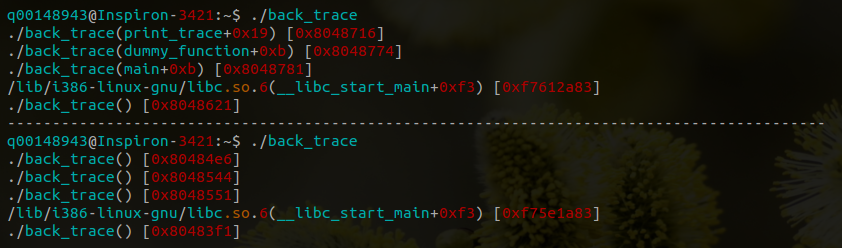
\includegraphics[width=0.92\textwidth]{backtrace.png}
  \caption{函数调用栈}
  \label{fig30}
\end{figure}

上面对rdynamic选项的基本功能及使用场景作了简要的说明。下面阐述为什么编译时加上rdynamic选项能达到这样的效果。
\begin{figure}[!htb]
  \setlength{\abovecaptionskip}{0pt}
  \centering
  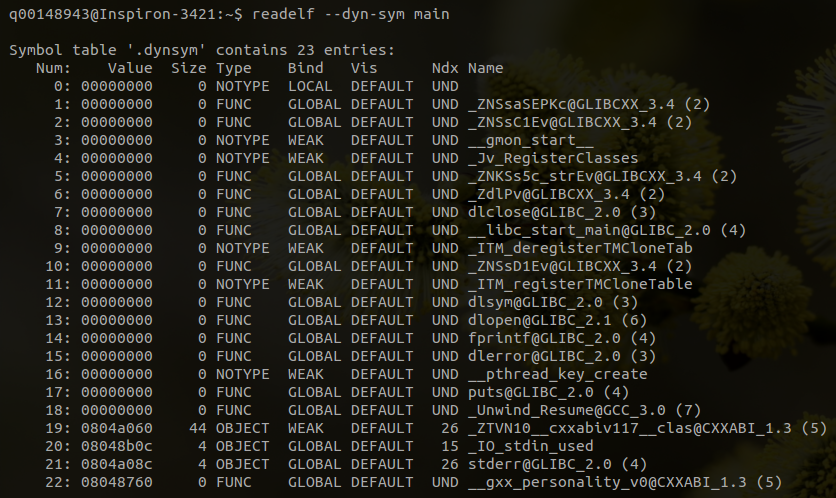
\includegraphics[width=0.92\textwidth]{nordynamic.png}
  \caption{不开启rdynamic}
  \label{fig31}
\end{figure}

从gcc的man手册可以知道,rdynamic选项的作用就是将目标链接程序的所有符号添加到程序的动态符号表\footnote{动态符号表就是动态链接器在解析符号时所要查找的表,如果表中存在某个待解析的符号,程序运行正常,否则上报undefined symbol。}中,这一点可以使用代码\ref{lst3}和readelf这一命令行工具来做验证。

readelf工具的--dyn-sym选项的功能就是显示ELF文件的动态符号表。代码\ref{lst3}不开启rdynamic选项编译后,使用readelf查看编译后二进制的动态符号表结果如图\ref{fig31}所示。

图\ref{fig32}是开启rdynamic选项后的结果。把图\ref{fig31}和图\ref{fig32}的结果作对比可以看出,开启rdynmic选项后,动态符号表中的记录多了21个entries,其中就包括类DataNode的成员函数及其它的一些函数,这就是开启rdynamic选项后能解析到类DataNode的构造函数的最根本原因。
\begin{figure}[!htb]
  \setlength{\abovecaptionskip}{0pt}
  \centering
  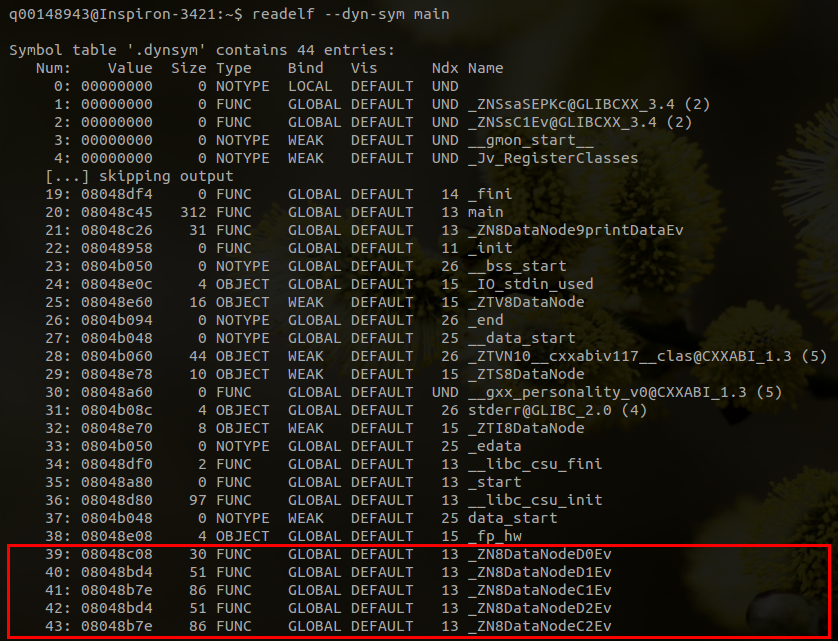
\includegraphics[width=0.92\textwidth]{rdynamic.png}
  \caption{开启rdynamic}
  \label{fig32}
\end{figure}


如果使用readelf -s查看一个二进制,结果会有两个符号表,如图\ref{fig33}所示。图中的.dynsym即是动态符号表,另一个则是符号表.symtab。这两个符号表的不同点如下:
\begin{itemize}
\item 动态符号表是符号表的子集;
\item loader加载二进制时会将动态符号表加载到内存,而符号表则不会加载到内存;
\item 动态符号表是给dynamic linker使用的,而符号表是给linker及debugger使用的。
\item 符号表可通过objcopy或strip命令从二进制中剥离,动态符号表则不可以,如果强制剥离,会导致二进制无法执行。
\end{itemize}
图\ref{fig34}演示了首先使用strip命令将二进制main的符号表剥离,然后执行,main运行正常;最后再通过strip命令将动态符号表剥离,再执行,则报错。
\begin{figure}[!htb]
  \setlength{\abovecaptionskip}{0pt}
  \centering
  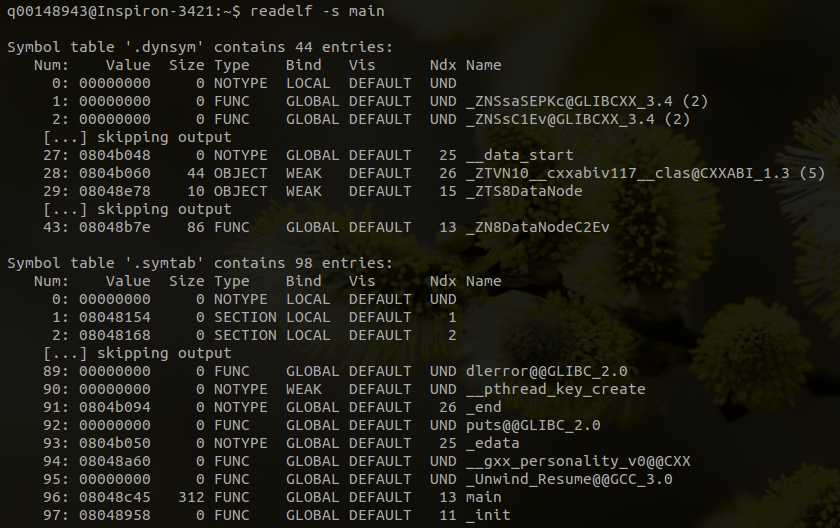
\includegraphics[width=0.92\textwidth]{both.png}
  \caption{符号表}
  \label{fig33}
\end{figure}

\begin{figure}[!htb]
  \setlength{\abovecaptionskip}{0pt}
  \centering
  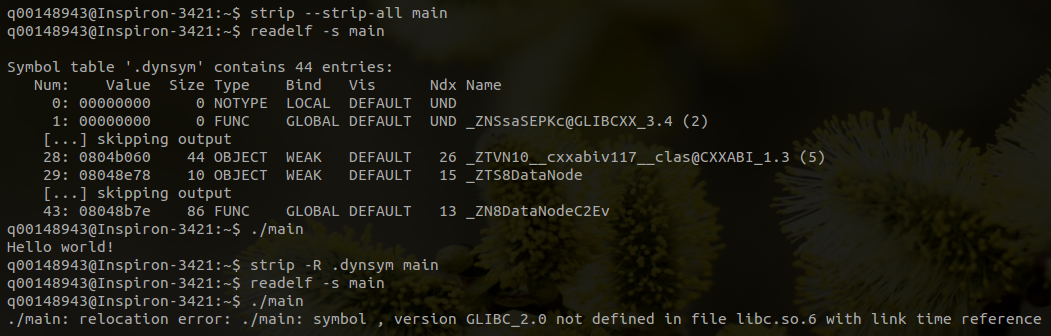
\includegraphics[width=0.92\textwidth]{strip.png}
  \caption{strip}
  \label{fig34}
\end{figure}

在本章节的最后,对代码\ref{lst5}中call指令后面的@plt作一点介绍性的说明。PLT,Procedure Linkage Table的缩写,是为解决动态库代码段不能共享而提出的一个概念。

代码\ref{lst5}的第20行即是代码\ref{lst4}第10行的汇编代码,该行汇编代码在执行时会直接跳转到Procedure Linkage Table的一个entry,即代码\ref{lst7}的第23行\footnote{call后面的地址是570,即代码\ref{lst7}的第23行。},假设是PLT的第n个entry,记为PLT[n]。第23行同样是一条jump指令,这次这条jump指令跳转到了GOT(Global Offset Table的缩写)的一个entry,假设是GOT[n]。第一次调用puts函数时,GOT[n]是指向PLT[n]的第二条指令的,即代码\ref{lst7}的第24行。第24行压栈了一个立即数,紧接着25行又是一条跳转指令,跳转的地址是520,即第7行,PLT[0]的第一条指令。PLT[0]比较特殊,它的功能就是解析出函数puts的真正地址并将该地址写到GOT[n]\footnote{因为是从puts函数的PLT跳转过去的,所以解析的是puts函数的地址,同理如果是从new函数的PLT跳转过去的,那解析出来的就是new的地址。},经过这样的一番折腾后,call puts@plt就转化成了对puts函数的调用。后续如果再调用puts函数,则不需要再经过dynamic loader来解析地址了,因为第一次解析完成后,puts函数的地址已经写到GOT[n],直接取出该地址调用即可,如图\ref{fig35}所示。
\begin{spacing}{1.0}
  \lstinputlisting[label=lst7,caption=PLT,language={[x86masm]Assembler}]{list/plt.s}
\end{spacing}

\begin{figure}[!htb]
  \setlength{\abovecaptionskip}{0pt}
  \begin{center}
    \begin{singlespace}
      \begin{tikzpicture}[auto, node distance = 5.5cm]
        \node (link) [rect,rectangle split parts=5,
        text width=2.5cm,
        rectangle split part fill={black!20!white,green!30!white,white!30!orange,white!30!orange,white!30!orange,white!30!orange,white!30!orange,white!30!orange,blue!40!green}] {
          \nodepart[height=2cm]{text}     {\footnotesize call}
          \nodepart[height=1cm]{two}    {\footnotesize PLT}
          \nodepart[height=0.5cm]{three}  {}
          \nodepart[height=0.5cm]{four}   {\footnotesize GOT}
          \nodepart[height=0.5cm]{five}   {}
        };


        \node[yshift=0.5cm] at (link.north) {\textbf{program}};

        \node[draw,minimum width=0.3cm, minimum height=0.1cm] (a) at ($(link.one east) + (-0.21cm,0)$) {};
        \node[draw,minimum width=0.3cm, minimum height=0.1cm] (b) at ($(link.two east) + (-0.21cm,0)$) {};
        \node[draw,minimum width=0.3cm, minimum height=0.1cm] (c) at ($(link.four east) + (-0.21cm,0)$) {};

        \draw [decorate,decoration={brace,amplitude=8pt,mirror}]
        ($(link.north west) + (-0.1cm,0)$) -- ($(link.two split west) + (-0.1cm,0)$) node [black,midway,xshift=-1.2cm,align=center]
        {\footnotesize text};

        \draw [decorate,decoration={brace,amplitude=8pt,mirror}]
        ($(link.two split west) + (-0.1cm,0)$) -- ($(link.south west) + (-0.1cm,0)$) node [black,midway,xshift=-1.2cm,align=center]
        {\footnotesize data};

        \draw[->] (a.center) to [bend left=50] (b.center);
        \draw[->] (b.center) to [bend left=50] (c.center);

        \node (exe) [right=2.5 of link,rect,rectangle split parts=5, text width=2.5cm,
        rectangle split part fill={black!20!white,green!30!white,white!30!orange,white!30!orange,white!30!orange,white!30!orange,white!30!orange,white!30!orange,blue!40!green}]
        {
          \nodepart[height=2cm]{text}     {\footnotesize routine}
          \nodepart[height=1cm]{two}      {\footnotesize PLT}
          \nodepart[height=0.5cm]{three}  {}
          \nodepart[height=0.5cm]{four}     {\footnotesize GOT}
          \nodepart[height=0.5cm]{five}     {}
        };

        \node[yshift=0.5cm] at (exe.north) {\textbf{library}};
        \node[draw,minimum width=0.3cm, minimum height=0.1cm] (h) at ($(exe.one west) + (+0.21cm,0)$) {};

        \draw [decorate,decoration={brace,amplitude=8pt}]
        ($(exe.north east) + (0.1cm,0)$) -- ($(exe.two split east) + (0.1cm,0)$) node [black,midway,xshift=0.4cm,align=center]
        {\footnotesize text};

        \draw [decorate,decoration={brace,amplitude=8pt}]
        ($(exe.two split east) + (0.1cm,0)$) -- ($(exe.south east) + (0.1cm,0)$) node [black,midway,xshift=0.4cm,align=center]
        {\footnotesize data};

        \draw [-latex,thick,rounded corners] (c.center) -| ($(link.two east) + (1cm,0)$) -| ($(link.two east) + (2cm,0)$) |- (h.center);

      \end{tikzpicture}
    \end{singlespace}
  \end{center}
  \caption{Loading}
  \label{fig35}
\end{figure}



前面说了,PLT是为了解决动态库的代码段不能在进程间共享引入的,那说明在未引入这个概念前,动态库也是可以工作的,只是工作方式略有不同。在编译libdatanode.so时,不指定-fPIC参数编译出来的lib库即是以进程间不能共享代码段这种方式工作的。

PIC,Position Independent Code的缩写,位置无关代码,即带了这个参数编译出来的动态库,被加载到进程的任何地址段都是可以正常工作的。

代码\ref{lst8}是代码\ref{lst4}不带-fPIC参数编译出来的动态库libdatanode.so中getNode函数的汇编代码,其中第16行即是调用puts函数\footnote{从这段代码很难直接的看出来这里就是调用puts函数,运行二进制main加载libdatanode.so再通过gdb反汇编getNode函数就可以很清晰的看出来。}。可以看出,这里的调用是直接call一个地址6ba,而不再是 call puts@plt了。很明显,main加载libdatanode.so后,6ba不可能是puts函数的地址,main在加载libdatanode.so之后,需要对call 6ba做重定位,使call后面的地址是真正puts函数的地址,如图\ref{fig36}所示。这就是为什么不加-fPIC选项编译出的动态库不能进程间共享的原因:一个进程加载了动态库,需要对动态库中的某些符号做重定位,会修改该动态库的代码段;而每个进程对动态库中的符号重定位的地址是不相同的,导致各个进程间不能共享同一个动态库的代码段。但加上-fPIC参数后,就有了PLT和GOT,有了这两个表后,解析函数的过程中修改的是各个进程的数据段\footnote{数据段本来各个进程就是独立的。},而不是动态库的代码段,所以多个进程是可以共享一份代码的。
\begin{spacing}{1.0}
  \lstinputlisting[label=lst8,caption=load time relocation,language={[x86masm]Assembler}]{list/load_time_relocation.s}
\end{spacing}

\begin{figure}[!htb]
  \setlength{\abovecaptionskip}{0pt}
  \centering
  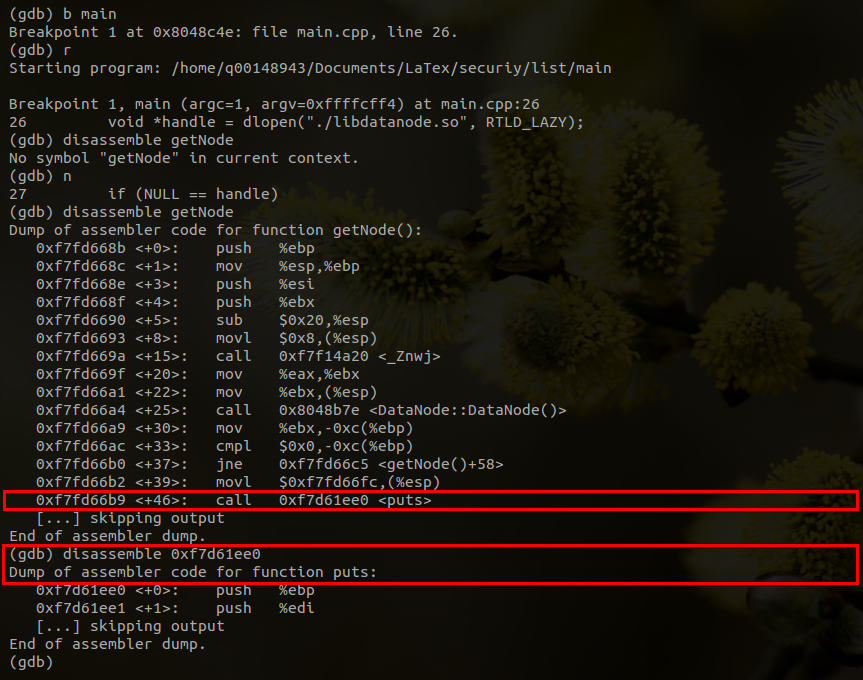
\includegraphics[width=0.92\textwidth]{gdb.png}
  \caption{gdb}
  \label{fig36}
\end{figure}

图\ref{fig37}是使用带-fPIC参数编译出的动态库同时被两个进程加载的内存布局示意图。图\ref{fig38}是不带-fPIC参数编译出的动态库同时被两个进程加载的内存布局示意图。从两图的对比中可以看出,不带-fPIC参数的动态库,不同的进程加载后,需要映射到不同的物理内存,即进程间不能共享同一物理内存中的该动态库。
\begin{figure}[!htb]
  \setlength{\abovecaptionskip}{0pt}
  \begin{center}
    \begin{singlespace}
      \begin{tikzpicture}[auto, node distance = 5.5cm]
        \node (link) [rect,rectangle split parts=8,
        text width=2cm,
        rectangle split part fill={black!20!white,white,green!50!white,white,white!30!orange,white!30!orange,white!30!orange,white}] {
          \nodepart[height=1.2cm]{text}     {\footnotesize kernel}
          \nodepart[height=0.3cm]{two}    {}
          \nodepart[height=1.0cm]{three}    {\footnotesize .so}
          \nodepart[height=0.5cm]{four}    {}
          \nodepart[height=0.3cm]{five}  {\footnotesize bss}
          \nodepart[height=0.4cm]{six}  {\footnotesize data}
          \nodepart[height=0.6cm]{seven}   {\footnotesize text}
          \nodepart[height=0.1cm]{eight}   {}
        };

        \node[yshift=0.5cm] at (link.north) {\textbf{\footnotesize virtual mem}};

        \draw [decorate,decoration={brace,amplitude=8pt,mirror}]
        ($(link.north west) + (-0.1cm,0)$) -- ($(link.text split west) + (-0.1cm,0)$) node [black,midway,xshift=-1.2cm,align=center]
        {\footnotesize 1GB};

        \draw [decorate,decoration={brace,amplitude=8pt,mirror}]
        ($(link.text split west) + (-0.1cm,0)$) -- ($(link.south west) + (-0.1cm,0)$) node [black,midway,xshift=-1.2cm,align=center]
        {\footnotesize 3GB};

        \node (exe) [right=4 of link,rect,rectangle split parts=8, text width=2cm,
        rectangle split part fill={black!20!white,white,green!50!white,white,white!30!orange,white!30!orange,white!30!orange,white}]
        {
          \nodepart[height=1.2cm]{text}     {\footnotesize kernel}
          \nodepart[height=0.3cm]{two}    {}
          \nodepart[height=1.0cm]{three}    {\footnotesize .so}
          \nodepart[height=0.5cm]{four}    {}
          \nodepart[height=0.3cm]{five}  {\footnotesize bss}
          \nodepart[height=0.4cm]{six}  {\footnotesize data}
          \nodepart[height=0.6cm]{seven}   {\footnotesize text}
          \nodepart[height=0.1cm]{eight}   {}
        };

        \node[yshift=0.5cm] at (exe.north) {\textbf{\footnotesize virtual mem}};

        \draw [decorate,decoration={brace,amplitude=8pt}]
        ($(exe.north east) + (0.1cm,0)$) -- ($(exe.text split east) + (0.1cm,0)$) node [black,midway,xshift=0.4cm,align=center]
        {\footnotesize 1GB};

        \draw [decorate,decoration={brace,amplitude=8pt}]
        ($(exe.text split east) + (0.1cm,0)$) -- ($(exe.south east) + (0.1cm,0)$) node [black,midway,xshift=0.4cm,align=center]
        {\footnotesize 3GB};


        \gettikzxy{(link.center)}{\linkx}{\linky}
        \gettikzxy{(exe.center)}{\exex}{\exey}

        \node[draw,minimum width=2cm, minimum height=1cm,fill=white!60!red] (so) at ($(\linkx/2+\exex/2,\exey)$) {\footnotesize .so};
        \node[yshift=0.5cm] at (so.north) {\textbf{\footnotesize physical mem}};

        \draw [dashed] (link.two split east) -- (so.north west);
        \draw [dashed] (link.three split east) -- (so.south west);

        \draw [dashed] (exe.two split west) -- (so.north east);
        \draw [dashed] (exe.three split west) -- (so.south east);
      \end{tikzpicture}
    \end{singlespace}
  \end{center}
  \caption{position independent code}
  \label{fig37}
\end{figure}


\begin{figure}[!htb]
  \setlength{\abovecaptionskip}{0pt}
  \begin{center}
    \begin{singlespace}
      \begin{tikzpicture}[auto, node distance = 5.5cm]
        \node (link) [rect,rectangle split parts=8,
        text width=2cm,
        rectangle split part fill={black!20!white,white,green!50!white,white,white!30!orange,white!30!orange,white!30!orange,white}] {
          \nodepart[height=1.2cm]{text}     {\footnotesize kernel}
          \nodepart[height=0.3cm]{two}    {}
          \nodepart[height=1.0cm]{three}    {\footnotesize .so}
          \nodepart[height=0.5cm]{four}    {}
          \nodepart[height=0.3cm]{five}  {\footnotesize bss}
          \nodepart[height=0.4cm]{six}  {\footnotesize data}
          \nodepart[height=0.6cm]{seven}   {\footnotesize text}
          \nodepart[height=0.1cm]{eight}   {}
        };

        \node[yshift=0.5cm] at (link.north) {\textbf{\footnotesize virtual mem}};

        \draw [decorate,decoration={brace,amplitude=8pt,mirror}]
        ($(link.north west) + (-0.1cm,0)$) -- ($(link.text split west) + (-0.1cm,0)$) node [black,midway,xshift=-1.2cm,align=center]
        {\footnotesize 1GB};

        \draw [decorate,decoration={brace,amplitude=8pt,mirror}]
        ($(link.text split west) + (-0.1cm,0)$) -- ($(link.south west) + (-0.1cm,0)$) node [black,midway,xshift=-1.2cm,align=center]
        {\footnotesize 3GB};

        \node (exe) [right=5 of link,rect,rectangle split parts=8, text width=2cm,
        rectangle split part fill={black!20!white,white,green!50!white,white,white!30!orange,white!30!orange,white!30!orange,white}]
        {
          \nodepart[height=1.2cm]{text}     {\footnotesize kernel}
          \nodepart[height=0.3cm]{two}    {}
          \nodepart[height=1.0cm]{three}    {\footnotesize .so}
          \nodepart[height=0.5cm]{four}    {}
          \nodepart[height=0.3cm]{five}  {\footnotesize bss}
          \nodepart[height=0.4cm]{six}  {\footnotesize data}
          \nodepart[height=0.6cm]{seven}   {\footnotesize text}
          \nodepart[height=0.1cm]{eight}   {}
        };

        \node[yshift=0.5cm] at (exe.north) {\textbf{\footnotesize virtual mem}};

        \draw [decorate,decoration={brace,amplitude=8pt}]
        ($(exe.north east) + (0.1cm,0)$) -- ($(exe.text split east) + (0.1cm,0)$) node [black,midway,xshift=0.4cm,align=center]
        {\footnotesize 1GB};

        \draw [decorate,decoration={brace,amplitude=8pt}]
        ($(exe.text split east) + (0.1cm,0)$) -- ($(exe.south east) + (0.1cm,0)$) node [black,midway,xshift=0.4cm,align=center]
        {\footnotesize 3GB};


        \gettikzxy{(link.center)}{\linkx}{\linky}
        \gettikzxy{(exe.center)}{\exex}{\exey}

        \node[draw,dashed,minimum width=4.7cm, minimum height=2cm,fill=white!90!green] (back) at ($(\linkx/2+\exex/2,\exey)$) {};
        \node[yshift=0.4cm] at (back.north) {\textbf{\footnotesize two physical mem for the same so}};

        \node[draw,minimum width=2cm, minimum height=1cm,fill=white!60!red] (so) at ($(\linkx/4+\exex/4,\exey) + (0.7cm,0)$) {\footnotesize .so};
        \node[draw,minimum width=2cm, minimum height=1cm,fill=white!60!red] (soso) at ($(3*\linkx/4+3*\exex/4,\exey) + (-0.7cm,0)$) {\footnotesize .so};

        \draw [dashed] (link.two split east) -- (so.north west);
        \draw [dashed] (link.three split east) -- (so.south west);

        \draw [dashed] (exe.two split west) -- (soso.north east);
        \draw [dashed] (exe.three split west) -- (soso.south east);
      \end{tikzpicture}
    \end{singlespace}
  \end{center}
  \caption{load time relocation}
  \label{fig38}
\end{figure}



\section{问题改进}
前面章节说了,如果代码\ref{lst3}在编译时不加rdynamic选项,二进制main在打开动态库时会报undefined reference,导致整个程序运行失败。那问题来了,PGW也给lib库提供了很多接口,在编译PGW时并没有带rdynamic参数,那么在PGW加载lib库时,这些提供给lib库的接口函数是如何解析成功的。

PGW当前的处理方式是:每新增一个lib库接口,就需要FE的lib库提供一个注册函数来注册这个接口,以这种方式告诉FE的lib库,PGW提供函数A,原型是prototypeA,地址是0xABCDEF。FE的lib库拿到这个地址后,直接强转成protoypeA类型的函数来使用。这种方式的一个最大好处就是效率高,因为FE的lib库拿到这个地址后,直接强转就可以使用,不需要经过多条指令来查找A函数的地址。但也有一个坏处就是,PGW每开放一个lib库接口,就需要FE的lib库对应的开发一个注册接口,同时PGW在初始化FE的lib库时,需要找到FE的该注册接口,并调用该接口将新开放的lib库接口注册给FE的lib库,绕晕没:)。

PGW初始化FE的lib库的代码有1K,其中有0.5K就是在找FE lib库中的注册函数来注册提供给FE的lib库接口的。在160版本引入了虚基类,以虚函数的方式来封装提供给FE的lib库接口,有效的遏制了初始化lib库的代码继续膨胀,同时也减轻了FE使用lib库接口的负担;但这种方式相比第一种,性能略有下降,因为每次函数调用都得先到虚函数表中查找接口函数的地址,然后才能真正调用这些接口,同时对各个版本的兼容性有了更高的要求,因为一旦虚函数表不匹配,很容易导致PGW进程重启。

还有一种方式就是编译PGW时加上rdynamic选项,这样PGW提供给FE的lib库接口,只要把相应的头文件发布给FE就可以了,不需要FE开发注册接口,FE使用这些接口,就和我们使用VPP组件的接口一样,看了函数原型就可以直接拿来用,这样对FE的开发人员来说也更“人性化”一些。这种方式的性能和使用虚函数是相当的,但对兼容性的要求没有使用虚函数高。唯一的不足就是加了rdynamic编译选项后,编译出的PGW二进制会稍大,运行时占用内存稍多,因为要加载动态符号表。在目前PGW二进制编译出来32M的情况下,加了该选项后,编译出的二进制在38M左右。


\end{document}
%%%%%%%%%%%%%%%%%%%%%%%%% 正文部分结束%%%%%%%%%%%%%%%%%%%%%%

